\documentclass{llncs}
\usepackage{subcaption}
\usepackage[T1]{fontenc}
\usepackage{float}
\usepackage{graphicx}
\setlength{\floatsep}{5pt}
\setlength{\textfloatsep}{5pt}
\setlength{\intextsep}{5pt}
\setlength{\abovecaptionskip}{2pt}
\setlength{\belowcaptionskip}{2pt}
\usepackage[sort]{cite}


\begin{document}
\title{Balanced Accuracy Evaluation of Machine Learning Models for Self-Made Photographic Documentation of Beekeeping Frames}
\author{Jakub Iwaszkiewicz}
\institute{Wrocław University of Science and Technology, Wrocław, Poland
\email{264506@student.pwr.edu.pl}\\}
\maketitle

\section{Introduction}
The beekeeping domain has been growing in recent years, providing
useful tools that allow beekeepers to replace traditionally employed
methods that are inaccurate and time consuming for the beekeeper.
These tools cover many types of technology \cite{ref_HADJUR2022106604}, based
on electronic devices \cite{ref_FLORES20191111},
sound analysis \cite{ref_UTHOFF2023107589}, and noninvasive imaging methods \cite{ref_RODRIGUEZLOZANO2024109573}. The latter type of tools are often
used to record the development of the brood and the areas of different cell types
in the brood combs.

\section{Research Scope}
The research aimed to examine the balanced accuracy of machine learning models, including Gaussian Naive Bayes \cite{ref_gnb_article}, Support Vector Machine \cite{ref_svm_article}, and the Convolutional Neural Network \cite{ref_deep_learning}. The objective was to check the effectiveness of these models in a multilabel classification task related to bee frame \cite{ref_beekeeper_handbook} analysis.
More specifically, the focus was on evaluating whether the models could exceed the balanced accuracy thresholds of 70- 80\% in this particular dataset, as a preliminary benchmark to determine whether continuing research in this direction is justified. Based on the results, future work could involve collaboration with a domain expert to define a more practical evaluation metric. This may also include incorporating advanced image processing techniques, such as segmentation, to improve the interpretability and accuracy of the model predictions.

\newpage

\section{Data}
The dataset used in this research consists of 434 self-collected and self-labeled photographs of bee frames. The dataset is highly imbalanced, the distribution is shown in Figure~\ref{fig2}. More than 80\% of the samples belong to the non-capped class, while fewer than 20\% belong to the capped class. Another bar graph in Figure~\ref{fig22_1} represents the distribution of bee frames containing honey, we can see that frames, which contain honey, are above 20\% of each photograph. In Figure~\ref{fig22_2}, the last distribution represents the hardness class which include of 10\% of low durable bee frame, above 80\% of bee frame ranked as medium and around 10\% of bee frames labeled as high durable. Each photograph includes three labels:
\begin{itemize}
  \item the presence of honey (true/false),
  \item the presence of cappings (true/false),
  \item the hardness of the comb (high/medium/low).
\end{itemize}
An example of the data is shown in Figure~\ref{fig1}.

\vspace{1em}

\begin{figure}[H]
\centering
\small
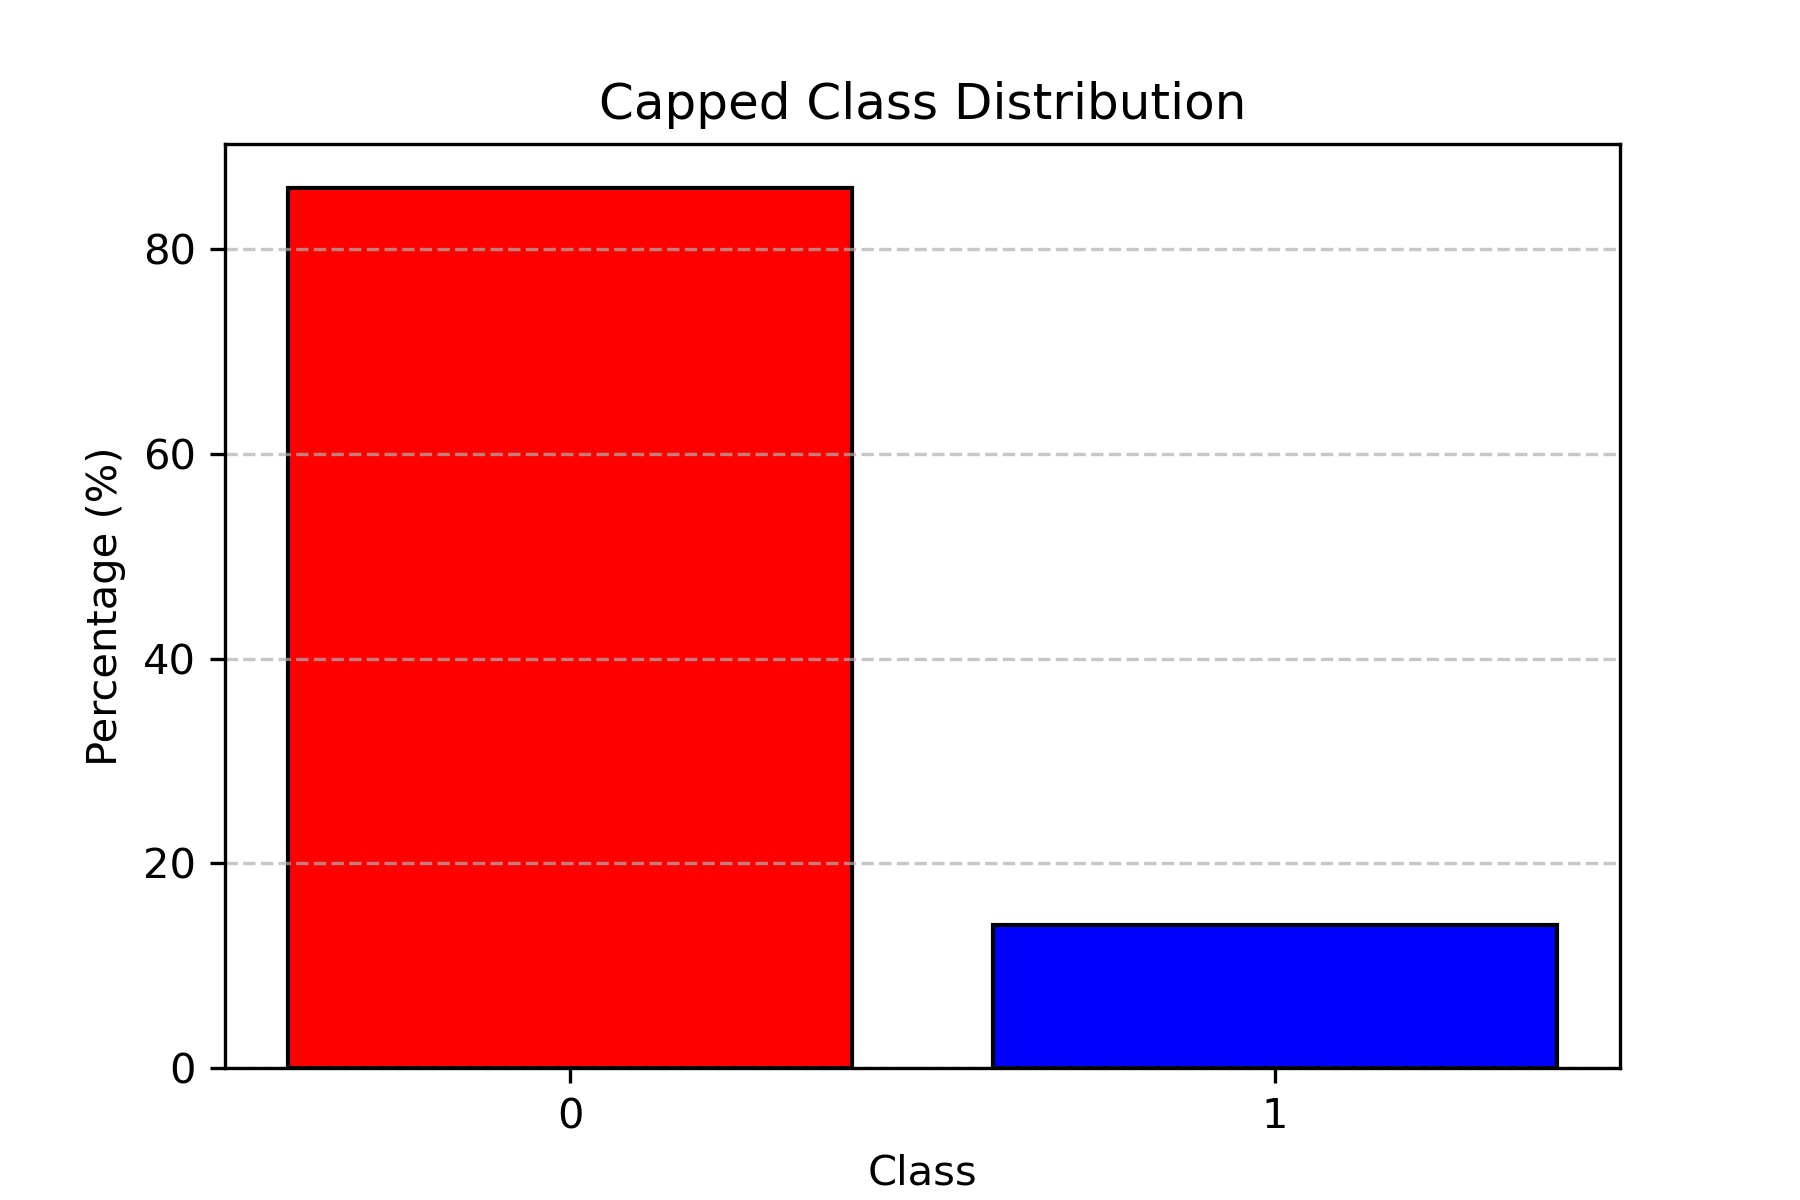
\includegraphics[width=0.75\textwidth]{Capped_class_distribution.png}
\caption{Class distribution of photos of capped frames. Class 0 (displayed in red) represents non-capped frames and class 1 (displayed in blue) represents capped frames.}
\label{fig2}
\end{figure}

\vspace{1em}

\begin{figure}
    \centering
    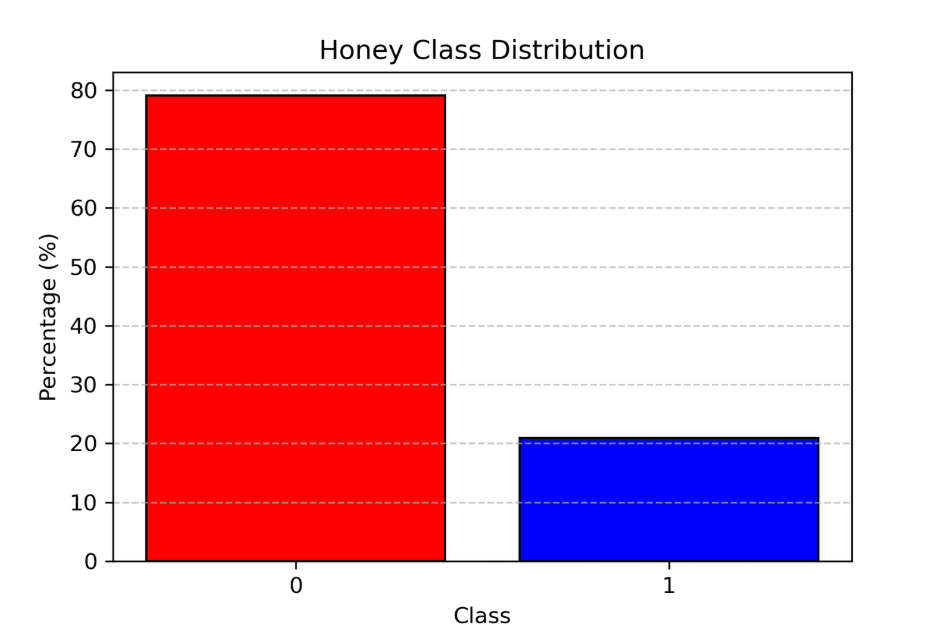
\includegraphics[width=0.75\linewidth]{dist_honey.png}
    \caption{Class distribution of photos of frames with or without honey. Class 0 (displayed in red) represents bee frames not containing honey and class 1 (displayed in blue) represents bee frames containing honey.}
    \label{fig22_2}
\end{figure}

\vspace{1em}

\begin{figure}
\centering
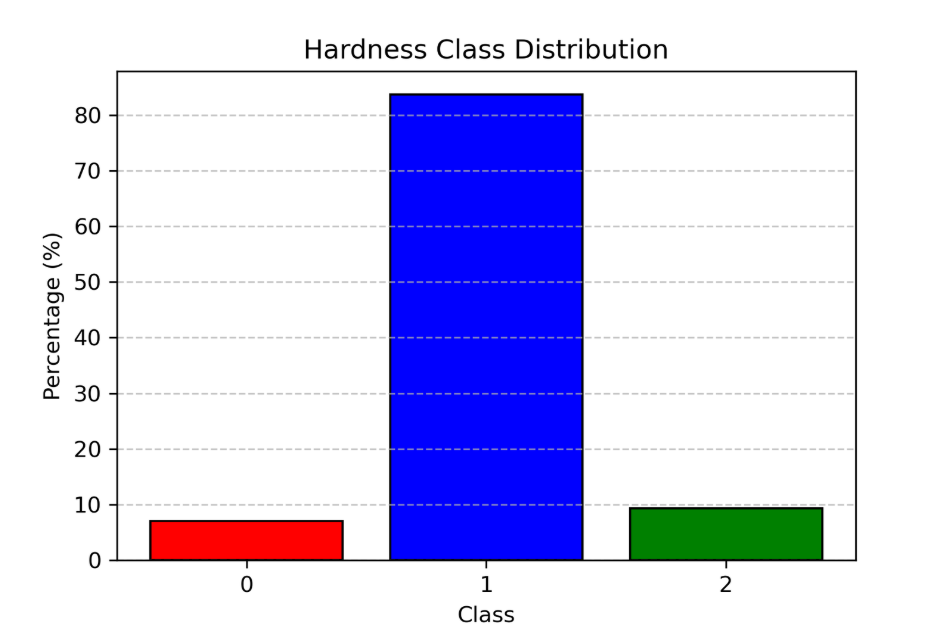
\includegraphics[width=0.75\linewidth]{dist_hardness.png}
\caption{Class distribution of photos of hardness levels frames. Class 0 (displayed in red) represents low hardness percent of bee frames, class 1 (displayed in blue) represents medium hardness percent of bee frames and class 2 (displayed in green) represents high hardness percent of bee frames.}
\label{fig22_1}
\end{figure}

\vspace{1em}

\begin{figure}[H]
\centering
\small
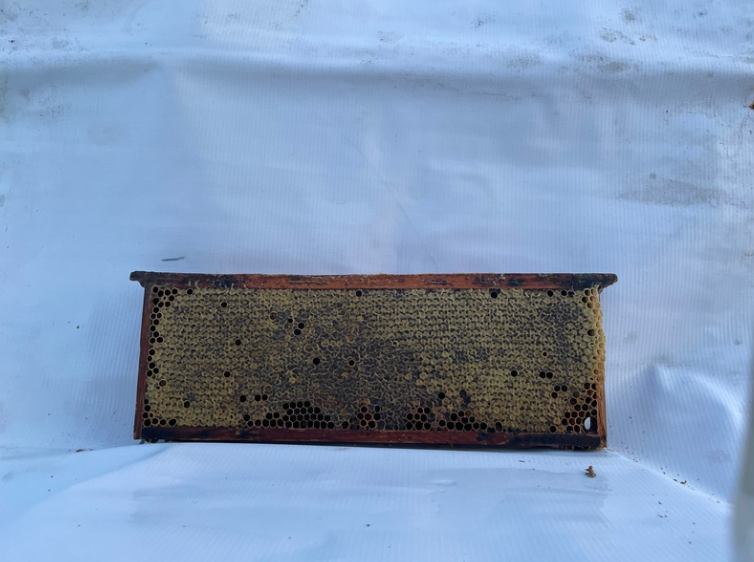
\includegraphics[width=0.75\textwidth]{example-bee-frame.png}
\caption{Example photo from the dataset. This bee frame labels would be: Cap - True, Honey - True and Hardness - High}
\label{fig1}
\end{figure}

\vspace{1em}







\section{Preprocessing}
To prepare the dataset for model training, several image preprocessing steps were applied. These transformations aimed to reduce bias, standardize input features, and make the data suitable for classical machine learning algorithms. The following steps were executed:
\begin{enumerate}
    \item Cropping to focus on relevant regions which can be seen in figure \ref{fig1_1}.
    \item Data augmentation to expand the dataset and minimize the bias related to sunlight, which can be seen in Figure \ref{fig1_2}.
    \item Separation into RGB color channels to reduce dimensionality.
    \item Application of the Histogram of Oriented Gradients (HOG) \cite{ref_hog_article} to each color channel which can be seen in Figure~\ref{fig1_3}.
    \item Flattening of the processed images to further reduce dimensionality and make the data suitable for linear models.
\end{enumerate}

\vspace{1em}

\begin{figure}[H]
\centering
\small
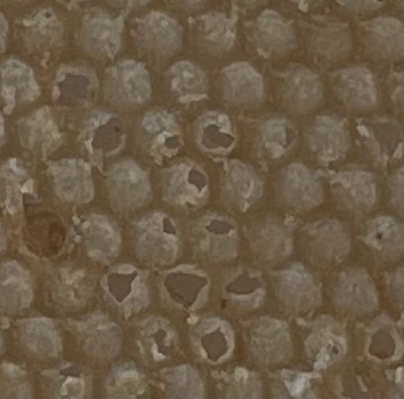
\includegraphics[width=0.70\textwidth]{example-of-cropped-bee-frame.png}
\caption{Example cropped photo from the dataset. This bee frame labels would be: Cap - False, Honey - False and Hardness - Low}
\label{fig1_1}
\end{figure}

\begin{figure}[H]
\centering
\small
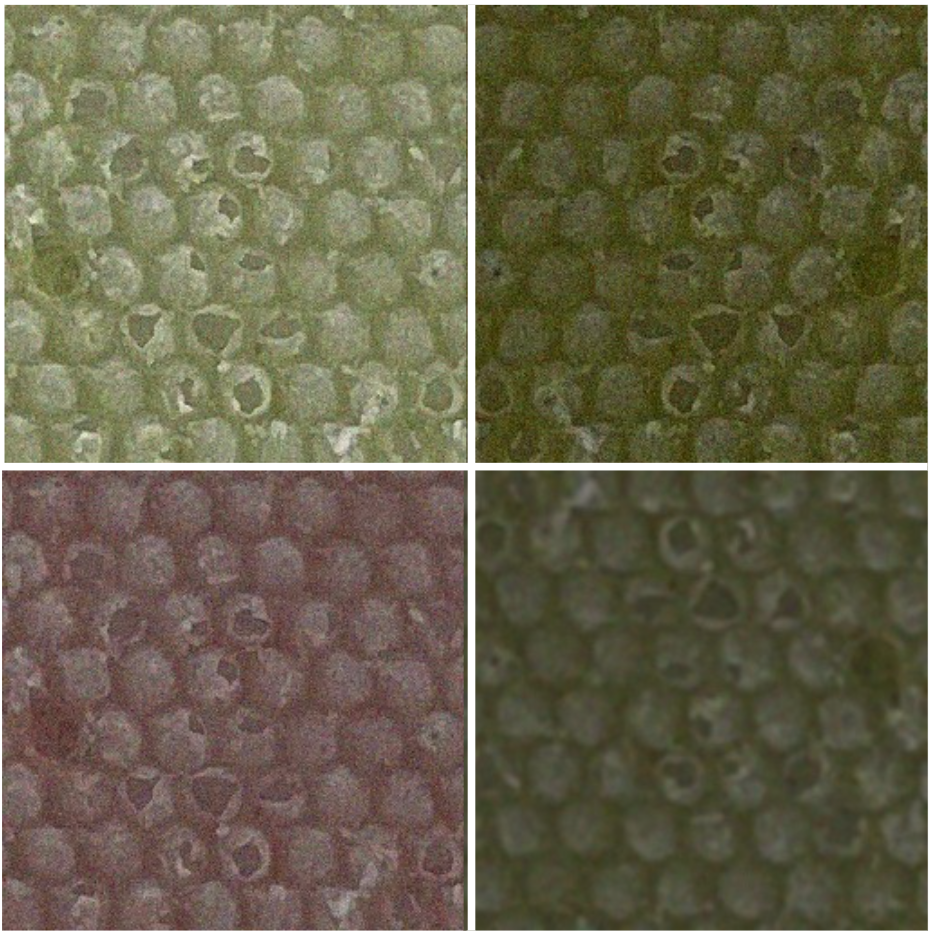
\includegraphics[width=0.70\textwidth]{example_of_augmented_bee_frame.png}
\caption{Example of few augmented photos from the dataset.}
\label{fig1_2}
\end{figure}

\begin{figure}[H]
\centering
\small
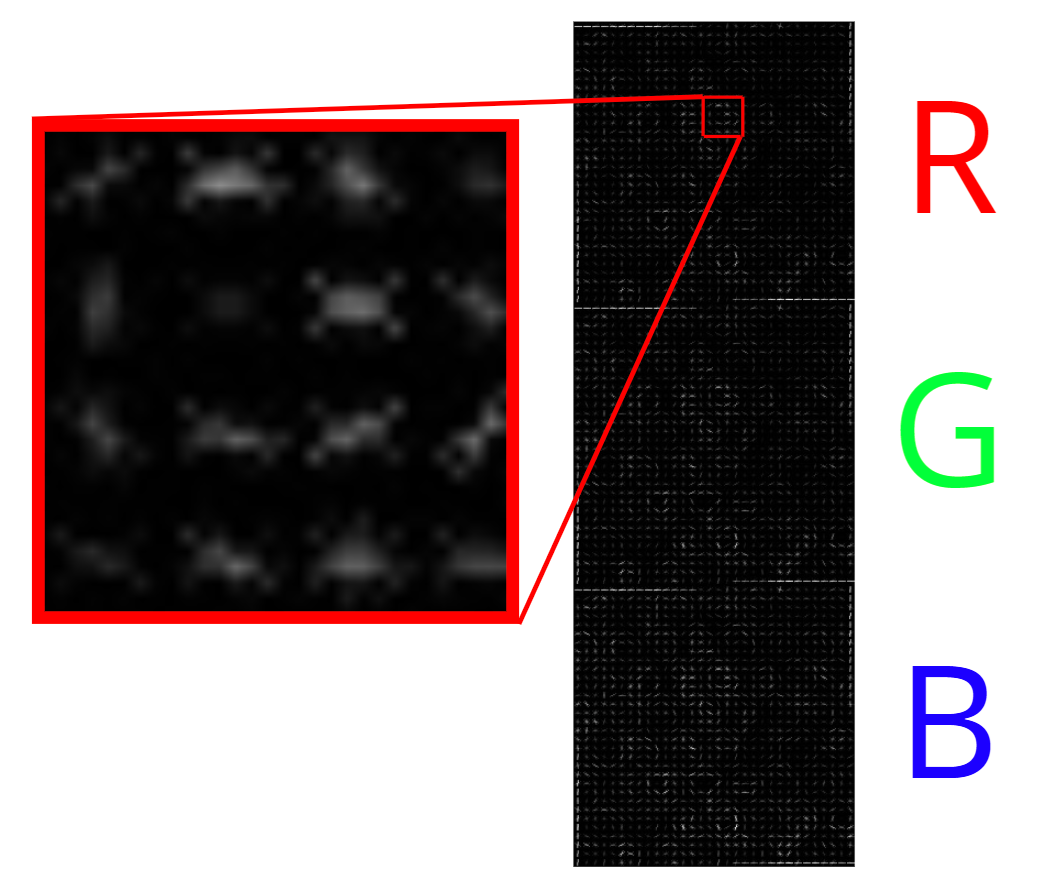
\includegraphics[width=0.70\textwidth]{visualization_how_photos_looks_after_augmentation.png}
\caption{Visualization how photos has been HOG computed and embedded by color channels.}
\label{fig1_3}
\end{figure}

\vspace{1em}



\section{Experimental Protocol}
The experiments were designed to evaluate model performance using balanced accuracy as the primary metric, which is well suited for scenarios of unbalanced data such as in the "hardness" label and does not disturb when the problem is binary. To ensure a reliable evaluation, a 5-fold stratified cross-validation strategy was used, preserving the distribution of labels between training and test splits.

\section{Results}
The experimental results show that the Gaussian Naive Bayes (GNB) model predicts more accurately both the Support Vector Machine (SVM) and the Convolutional Neural Network (CNN) in balanced accuracy metric, particularly for the "capped" label.

In Figure~\ref{fig4}, each group of bars represents the performance of the three models across five cross-validation folds. The GNB model (blue bars) consistently achieved the highest accuracy in all folds, with an average balanced accuracy of 0.875 and a standard deviation of 0.052, indicating relatively high and stable performance. The SVM model (orange bars) performed moderately well, achieving an average of 0.630 with higher variability ($\sigma$ = 0.066).

Further insights are provided in Figure~\ref{fig3}, where the performance of Gaussian Naive Bayes is divided by each label: Capped (blue), Honey (red), and Hardness (purple). Once again, the Capped label achieved the highest scores across folds, in some cases exceeding 0.90, confirming that the GNB is relatively highly effective in predicting this label. The honey label also produced strong results with a mean balanced accuracy of 0.779 and low variance ($\sigma$ = 0.013), demonstrating that the model reliably identified the presence of honey in the frames. However, GNB struggled with the Hardness label, achieving only 0.413 on average and showing more variability across folds ($\sigma$ = 0.056). This suggests that the visual characteristics associated with comb hardness are more ambiguous or inconsistently labeled, and might not be well captured by the current preprocessing approach.

\begin{figure}[H]
\centering
\small
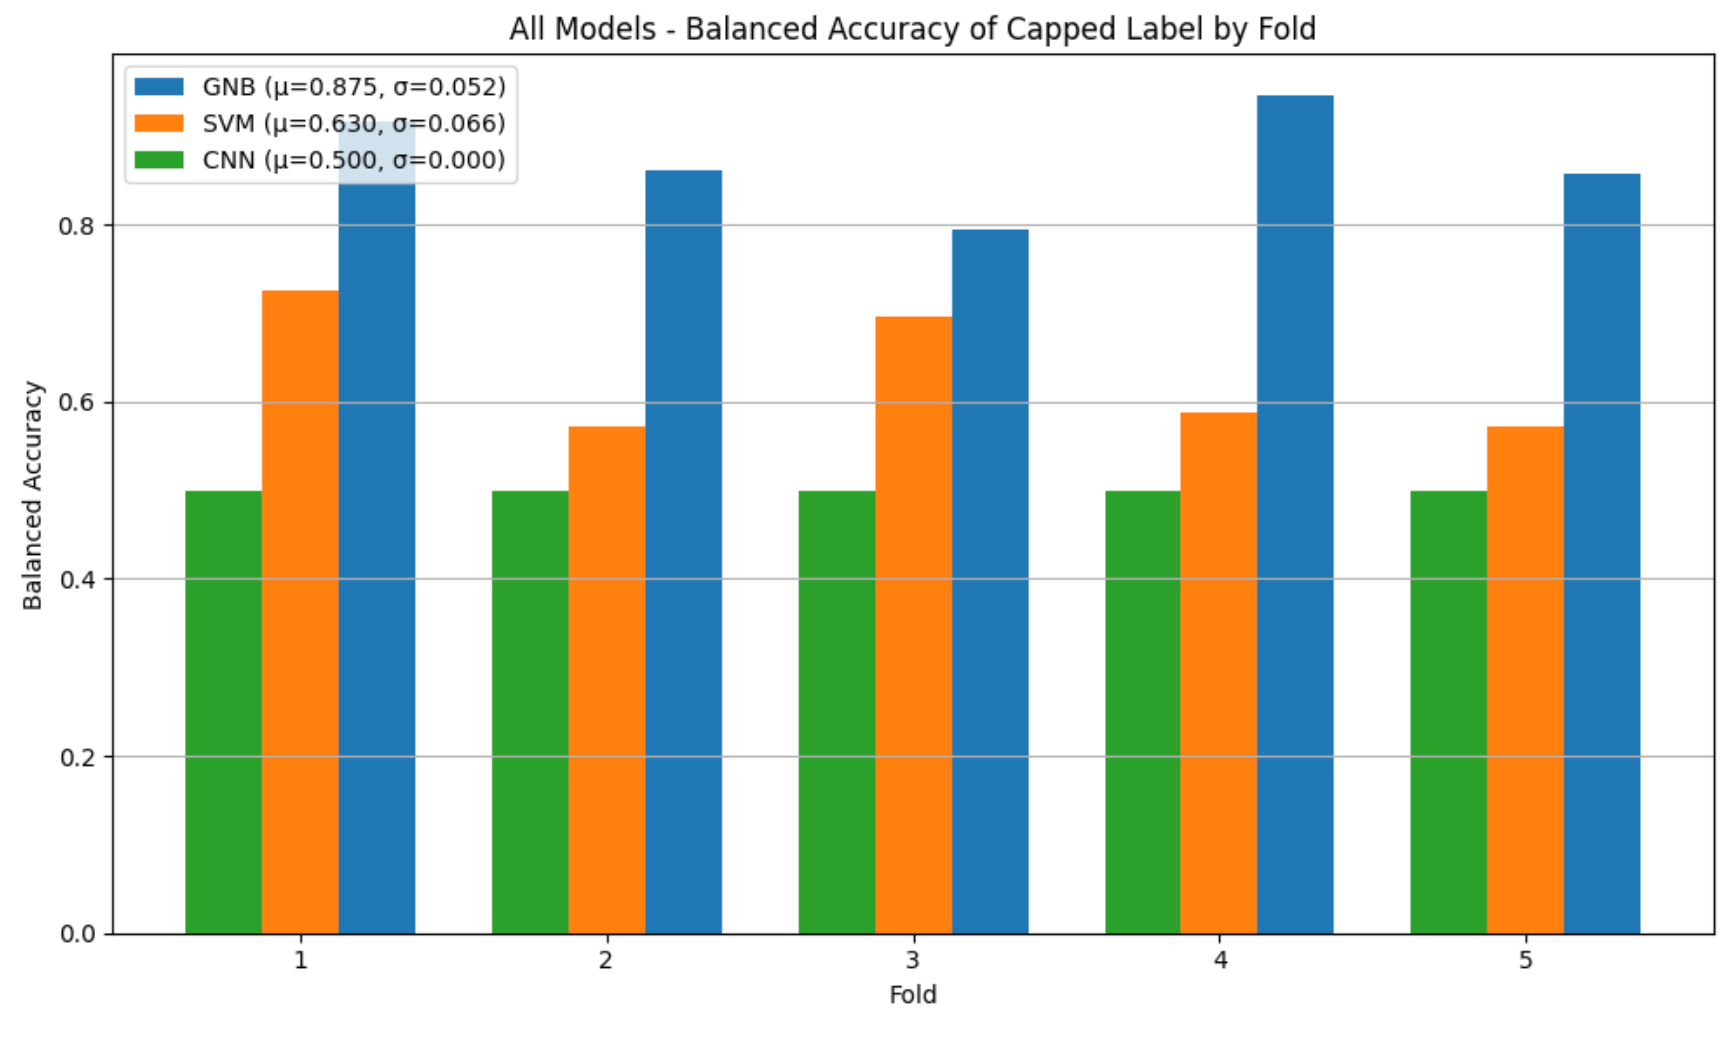
\includegraphics[width=0.75\textwidth]{isw/all-models-balanced-accuracy-of-capped-label-by-fold.png}
\caption{Balanced accuracy across five cross-validation folds for the presence of cappings classification task of all model: Gaussian Naive Bayes (displayed on blue), Support Vector Machine (displayed on orange color), convolutional neural network based on modified LeNet-5 architecture \cite{ref_lenet_5} (displayed on green color).}
\label{fig4}
\end{figure}

\begin{figure}[H]
\centering
\small
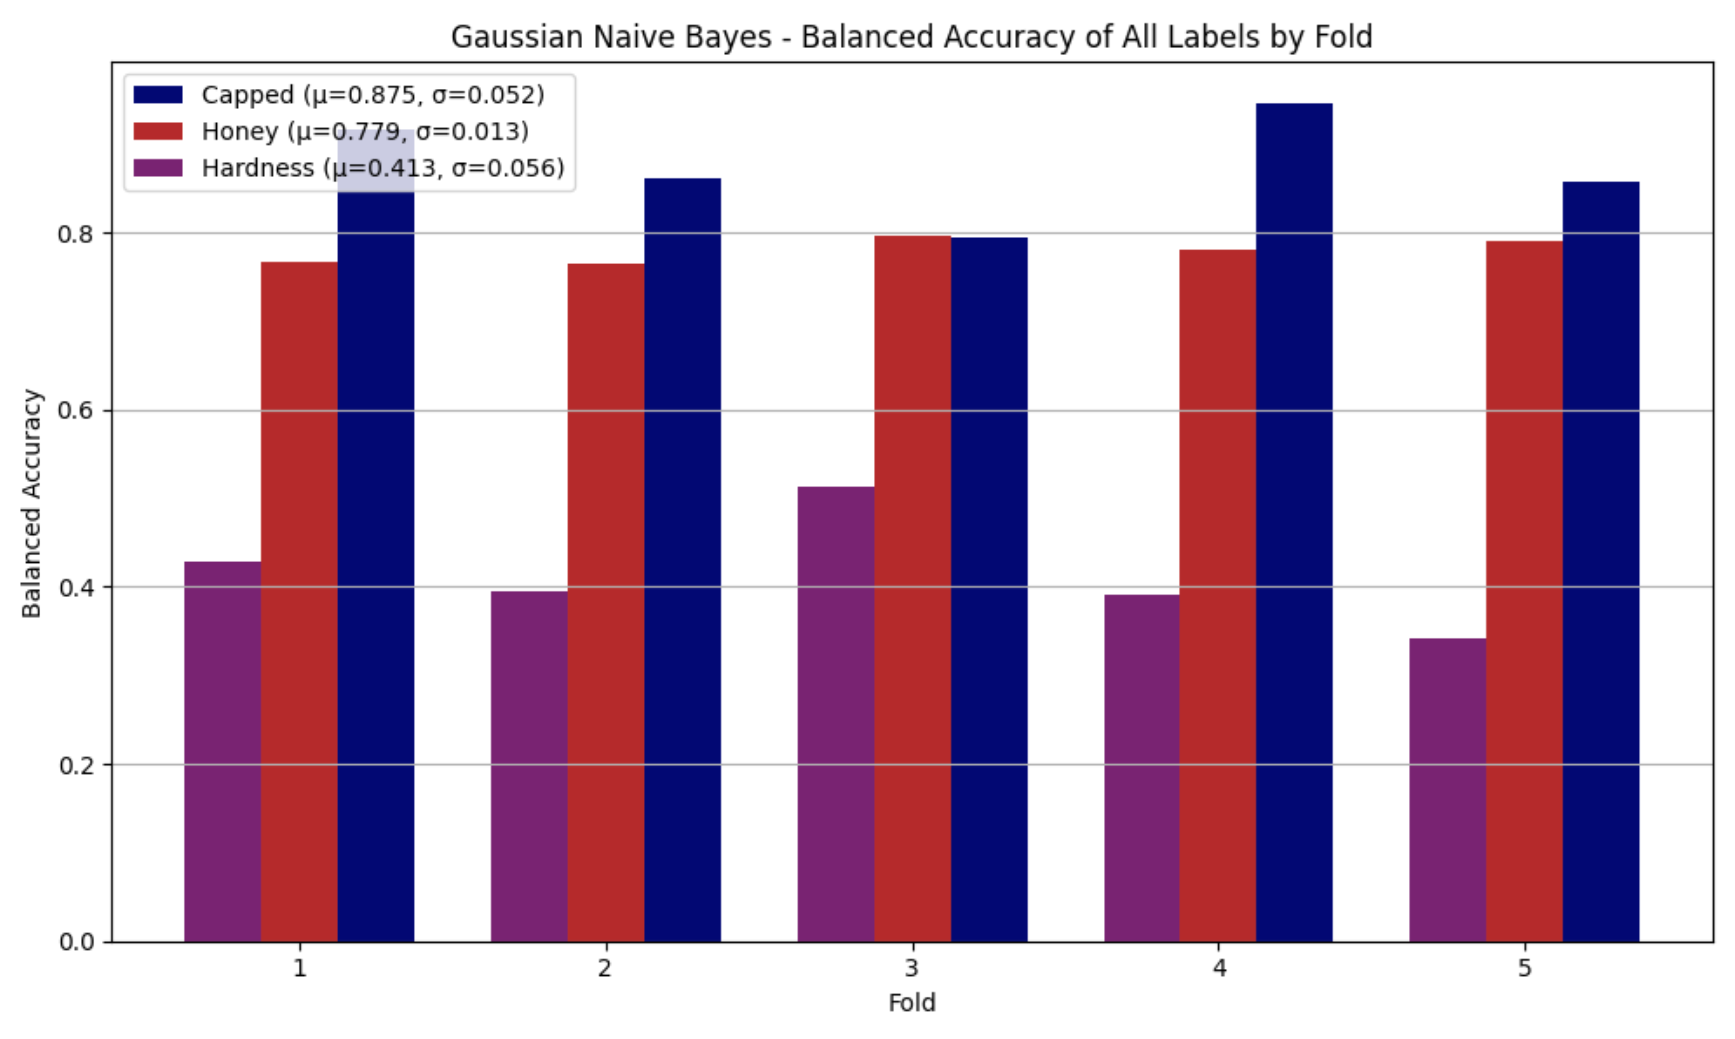
\includegraphics[width=0.75\textwidth]{isw/gnb-balanced-accuracy-of-all-labels-by-fold.png}
\caption{Balanced accuracy of the Gaussian Naive Bayes model across five cross-validation folds for three classification tasks: the presence of cappings (displayed on navy color), the presence of honey (displayed on red color), hardness level (displayed on purple color).}
\label{fig3}
\end{figure}

\section{Conclusion}

The results highlight that deep neural networks are not universally superior. Although convolutional neural networks (CNNs) are often praised for their performance in visual tasks, this experiment revealed that simpler models such as Gaussian Naive Bayes (GNB) outperformed CNNs in this dataset and in terms of balanced accuracy for the specific multilabel classification problem of bee frame analysis.

Specifically, GNB achieved relatively high and stable results on the 'capped' and 'honey' labels. On the other hand, the CNN model produced a flat balanced accuracy of 0.50 on the 'capped' label, indicating that decision of it is random.

\subsection*{Future Work}

Future work will focus on investigating the underperformance of the CNN model, particularly its inability to learn meaningful patterns for the 'capped' label. This will involve examining factors such as image resolution, network architecture, and preprocessing strategies like color normalization and augmentation. Since CNNs typically excel in visual tasks under the right conditions, this gap in performance suggests a need to re-evaluate the experiment. Further experiments will narrow the focus exclusively to the 'capped' class, aiming to improve results through techniques such as region-based segmentation. In parallel, collaboration with a domain expert will support the development of a more nuanced and practically useful evaluation metric. Rather than relying solely on balanced accuracy, which may miss the spatial and contextual subtleties of beekeeping, this new metric could incorporate criteria such as the accuracy of segmented capped areas, prediction consistency across similar frames, or weighting based on expert-defined zones of importance within each image. Such an approach would produce a more informative and application-relevant evaluation metric.

\vspace{1em}



\bibliographystyle{splncs04}
\bibliography{references}


\end{document}